\subsection{Das Starburst Project}

Das Starburst Projekt \cite{lohman1988Starbust}, \cite{haas1989extensible}, vorangetrieben und entwickelt von IBM,  startete unter der Prämisse, dass bestehende DBMSe nicht in der Lage sind den wachsenden Anforderungen von verschiedenen, neuartigen Applikationen vollumfänglich zu entsprechen. Zur Erfüllung der individuellen Ansprüche wurde das Starburst Projekt begonnen. Sein Ziel ist es dem \ac{DBI} die Möglichkeit zu geben, die relationale Datenbank zu erweitern und so die Bedürfnisse von spezifischen Anwendungen zu erfüllen. Beispielsweise ist es möglich, neue Zugriffs- und Speichermethoden zu implementieren oder neue Join-Methoden zu erstellen. Um diese Features zu ermöglichen, stellt Starbust eine Anfragesprache (Hydrogen), einen regelbasierten Optimierer, Query Rewriter und ein Ausführungssystem basierend auf relationaler Algebra zur Verfügung.


\subsubsection{Ausführung einer Anfrage}

Bei der Ausführung einer Anfrage mit Hilfe von Starburst wird grob zwischen zwei Phasen unterschieden: Übersetzungs- (Compile-) und Ausführungszeit (Run-Time) \cite{haas1989extensible}. Während der Compile-Time wird aus der Anfrage ein Plan generiert, der zur Run-Time durch das Execution System ausgeführt wird. Der Query Optimizer findet seine Anwendung zur Compile-Time; die Query Execution Engine kommt zur Run-Time zum Einsatz.

Der Ablauf der Ausführung (vgl. \ref{StarburstFlow}) ist vergleichbar mit dem Ablauf anderer Systeme.

\begin{figure}[ht]
  \centering
  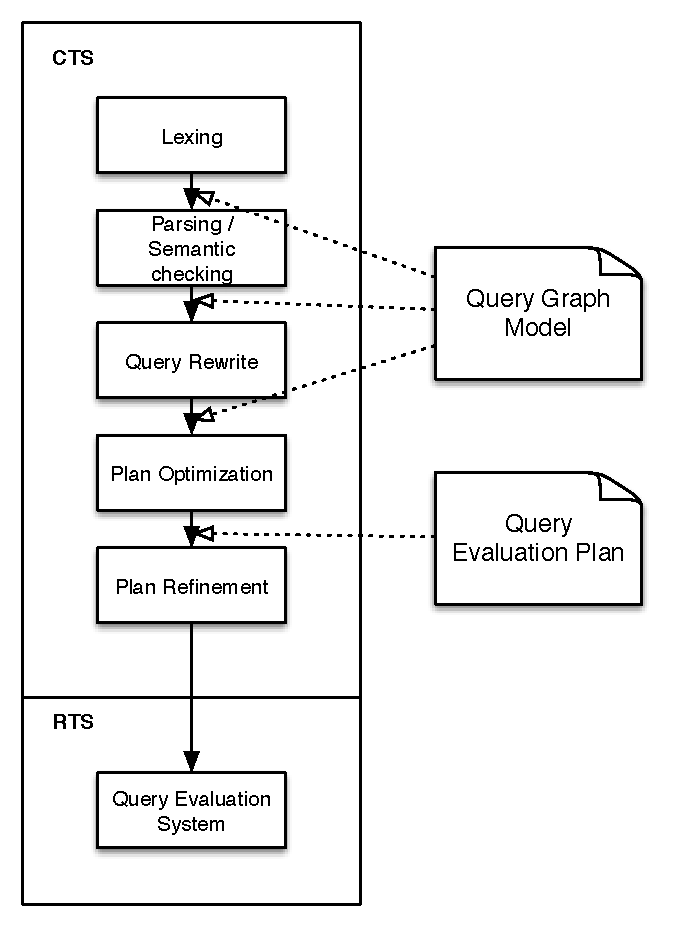
\includegraphics{02_Related_Work/StarburstFlow.pdf}
  \caption{Starburst}
  \label{StarburstFlow}
\end{figure}

Zur Compile-Time wird eine gegebene Anfrage - die Anfrage ist in Hydrogen (ähnlich SQL) formuliert - auf semantische Korrektheit geprüft und in ein \ac{QGM} übersetzt.

Der wichtigste Teil eines \ac{QGM} ist der Select-Operator. In diesem findet sich eine Projektionsliste und das Anfrageprädikat in Graphform. Die Knoten des Graphen referenzieren Relationen oder weitere \ac{QGM}-Operatoren. Mengenbegrenzungen\todo{was ist das?} tragen zur Erzeugung des Ergebnisses eines Operators bei, Quantoren zu dessen Einschränkung. Die Kanten des Graphen sind mit Predikaten wie insert, update, intersection, union oder group-by markiert. Neben dem Graphen enthält das \ac{QGM} auch aus Schema- und statistische Informationen. 

Basierend auf diesem \ac{QGM} wird die Optimierung der Anfrage zuerst durch einen Query Rewriter, einen Plan Optimierer und einen Plan Refiner durchgeführt.

Der Query Rewriter hat zwei konkrete Aufgaben: Auf der einen Seite soll die Anfrage in eine möglichst deklarative Form umgewandelt werden, hierbei werden insbesondere Anfragen entschachtelt. Auf der anderen Seite sollen weithin in der Forschung akzeptierte Heuristiken, beispielsweise der Push-Down von Argumenten, angewandt werden.


Bei der Planoptimierung durchläuft der Plan vom \ac{QGM} hin zu einem QEM drei Stationen. Die drei wesentlichen Aspekte sind der Plan Generator, die Berechnung der Plankosten, um den optimalen Plan auszuwählen. 

\subsubsection{Regel-Maschine}

Zur Ausführung von Transformationen wurde für die Starburst Datenbank eine eigene Regel-Maschine entwickelt \cite{lohman1988Starbust}. Diese Regelmaschine ist für die Anführung von Regelsets verantwortlich. Die Regeln lassen sich in drei Klassen einteilen:

\begin{itemize}
\item Migration von Prädikaten
\item Migration von Projektionen
\item Verschmelzung von Operationen
\end{itemize}



Die Regelmaschine basiert auf fünf Prinzipien:

\begin{enumerate}
\item Regel der arbiträren Komplexität: Eine Regel ist bei Starburst in zwei Teile aufgeteilt: Eine Koordinierungs- und eine Ausführungsfunktion. Bei dem Aufruf einer Regel muss zuerst geprüft werden, in wie weit die Regel angewendet werden darf. Ist sie anwendbar, wird die Ausführungsfunktion exekutiert.

\item Bei der Nutzung eines \ac{QGM} kann entweder eine Tiefen- als auch eine Breitensuche zur Anwendung kommen. Diese Art der Suche ist weder an die Regel noch an das Regelset geknüpft, sondern mit dem QGM selbst verbunden.


\item Die Regeln werden bei Starburst in Regelsets unterteilt. Ein Regelset besteht aus mehreren Regeln, die entweder sequenziell nach einer vorab vergebenen Priorität oder einem statistischen Verfahren aufgerufen werden. Jede Regel und jedes Regelset kann andere Regeln und Regelsets als Teil einer Subroutine ausführen. Neben der Funktion der Zusammenfassung der Regeln ist dies Aufgabe der Regelsets.

\item Um die Ausführung von Transformationen zu limitieren, insbesondere bei der Ausführung des Rewriters, kann ein Budget vorgeschrieben werden. Sobald dieses Zeitbudget aufgebraucht ist, wird die Ausführung von Regeln abgebrochen. Es ist für diese Funktion unbedingt notwendig, dass Regeln immer vollständige QGMs zurückliefern, da sonst ein unvollständiger QGM als Resultat des Optimierers entstehen kann.

\item Schlussendlich ist es dem Nutzer der Datenbank möglich zu jedem beliebigen Zeitpunkt Regeln außer Kraft zu setzen. Dies geschieht nur für den Nutzer lokal andere Nutzer der Datenbank sind nicht betroffen. Spezielle Anwendungsfälle können so passgenau optimiert werden.
\end{enumerate}

\subsubsection{Plan Optimierer}

Der Plan Optimierer selbst ist regelbasiert nutzt aber nicht den transformierenden, sondern einen generierenden Ansatz. Mit Hilfe von Basisoperatoren sog. \ac{LOLEPOP}s werden mit Hilfe von Regeln sog. \ac{STAR}s Pläne erzeugt. Die Basisoperatoren \ac{LOLEPOP}s bilden einfach Operationen wie SCAN und SORT. Ein Plan besteht aus mehreren dieser \ac{LOLEPOP}s, die gemeinsam einen Plan ergeben.

Der \ac{STAR} definiert ein bekanntes parametrisiertes Objekt. Es besteht aus einer Bedingung zur Anwendbarkeit und einer Definition  eines Plans. Ist ein STAR auf einen Teilplan anwendbar, wird dieser STAR an dieser Stelle referenziert. Der Plan selbst hat einen rootSTAR als Startpunkt. Mit Hilfe der STARs\todo{Stil} innerhalb des \ac{QGM}s ist eine Grammatik mit deren Hilfe alternative Pläne zu finden sind. 

Bei der Zusammensetzung von verschiedenen alternativen Plänen kommt ein Gluemechanismus zu Einsatz. Er verhindert, dass die Anzahl der Alternativen die in Plänen vorkommen vervielfacht werden. So entstehen aus GQMs QEPs deren Kosten geschätzt werden können.

